\documentclass[conference]{IEEEtran}
\IEEEoverridecommandlockouts
% The preceding line is only needed to identify funding in the first footnote. If that is unneeded, please comment it out.
\usepackage{amsmath,amssymb,amsfonts}
\usepackage{algorithmic}
\usepackage{graphicx}
\usepackage{float}
\usepackage{booktabs}
\usepackage{textcomp}
\usepackage{listings}
\usepackage{hyperref}
\usepackage{siunitx}
\usepackage[T1]{fontenc}
\usepackage[utf8x]{inputenc}
\def\BibTeX{{\rm B\kern-.05em{\sc i\kern-.025em b}\kern-.08em
    T\kern-.1667em\lower.7ex\hbox{E}\kern-.125emX}}
\begin{document}

\lstset{basicstyle=\footnotesize\ttfamily,breaklines=true,literate={á}{{\'a}}1 {ê}{{\^e}}1 {é}{{\'e}}1 }

\title{Topic categorization in Portuguese news articles\\
\thanks{Fundação para a Ciência e Tecnologia} }


\author{\IEEEauthorblockN{André F. Santos}
\IEEEauthorblockA{\textit{CRACS \& INESC-Porto LA} \\ \textit{Faculty
of Sciences, University of Porto}\\ Porto, Portugal \\
afs@inesctec.pt} }

\maketitle

\begin{abstract}
Categorizing news articles according to their contents allows to
decrease the information entropy in a world where the rate of
publication of digital text documents is increasing fast. In this
article we describe ongoing work which aims to evaluate the
feasibility of implementing a classifier which is lightweight
enough to be used in real time on the client side of a web
application.  More specifically, we gathered a corpus of Portuguese
news and used it to train and evaluate several classification
algorithms. We analyze the results obtained in terms of the
classifiers error rate, training time and memory footprint.
\end{abstract}

\begin{IEEEkeywords} topic categorization, machine learning, text
mining \end{IEEEkeywords}

\section{Introduction}
Online news articles first appeared as reprints from traditional
newspapers; nowadays, however, they represent now the primary source
of news for some segments of the population, both in developed and
developing countries (whether consumed directly in the newspaper
website, or indirectly e.g. through a social media application or a
feed catcher)\cite{greer2006evolution,boczkowski2005digitizing,chyi1999access}.

Unofficially know as \emph{the fourth branch of government}, the press
plays a vital role within our society, keeping us informed about
the current state of affairs (at a local and global scale) and acting
as a watchdog for the other three branches (legislative, executive and
judicial). The (lack of) freedom of press and access to the news in a
given country is even often considered an indicator of a lack of
democracy\cite{goode2009social,house2009freedom}.

As such, improving the ways citizens can access the information (view
it, query it and search it) contained in news articles has the
potential to contribute for a more informed and, ultimately, a
better society\cite{bollinger1988tolerant}.

On the other hand, the last decades have witnessed a fast increase on
the rate of publication of digital text documents. Traditional
document types, such as news articles, scientific papers or books are
now published online together with new formats, such as blog posts or
tweets, each having thousands or millions of new documents published
each day\cite{hilbert2011world,allan2006online}.

And it was not only the publication step which has moved to the
digital world; in fact, most often nowadays the whole document
lifecycle happens digitally, with virtual tools available for
researching, writing, styling, publishing and sharing\cite{williams2009personal}.

Having the entire workflow happening within the digital world presents
some opportunities when compared to the traditional
process\cite{o1997comparison}. In particular, due to the current
processing power commonly available, tasks related to the manipulation
of the information contained within these documents (searching,
compiling, annotating, sharing, \dots) can now be performed
automatically and targeting a large amount of articles.

In addition to the document content (for example, in a news article,
the \emph{title}, \emph{lead} and \emph{body}), its metadata is also
important: author(s), date of publication, source, topic, mentioned
entities and their relations, etc\cite{yaginuma2003metadata,yaginuma2003design}. Some of
this metadata might be filled in and stored along with the document
(e.g. \emph{author} and \emph{date of publication}); other is usually
extracted from the document content (e.g. mentioned
entities)\cite{vadrevu2005automated}.

An example of a feature which improves information access is the
categorization of news articles by the topic (or topics) of its
content\cite{kim2006extracting}. The presence of such a categorization
may influence the way the information is stored, organized, displayed
and queried\cite{teitler2008newsstand}.

\begin{figure}[htbp]
\centerline{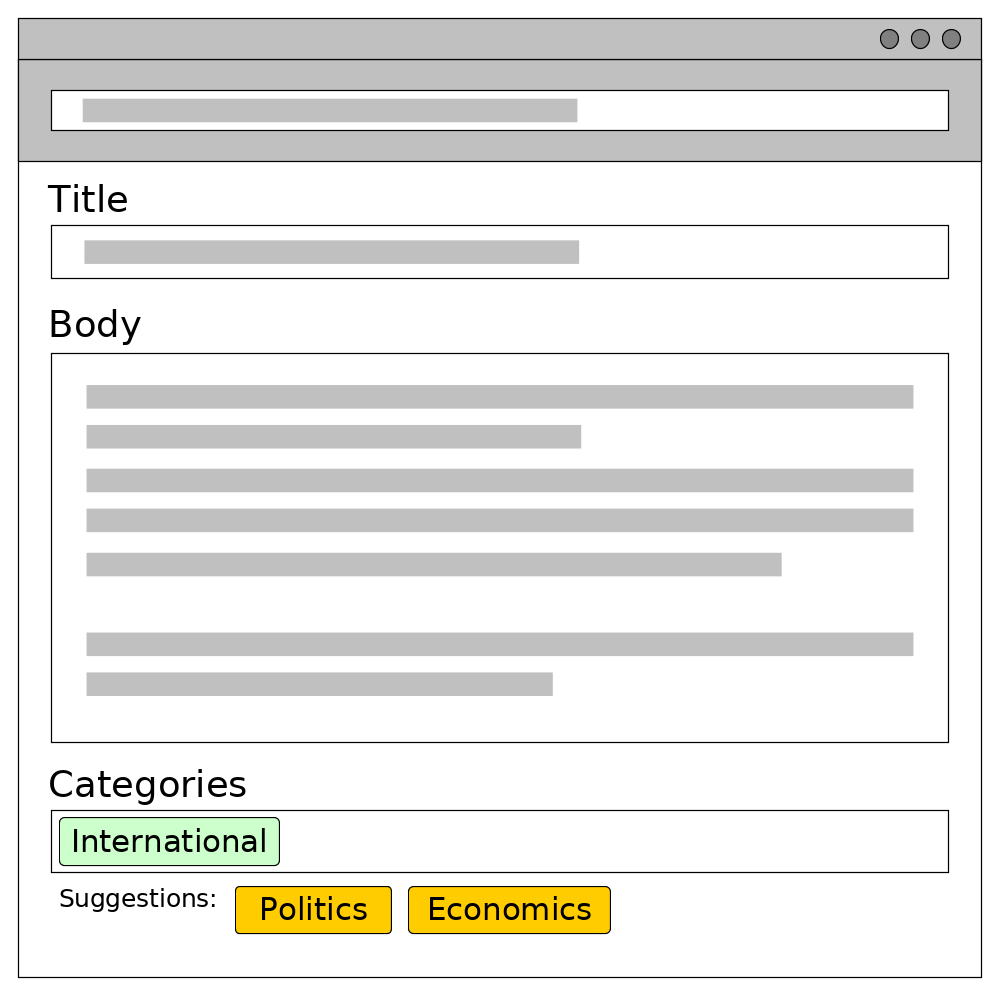
\includegraphics[width=.97\columnwidth]{imgs/wireframe}}
\caption{Category classification and suggestion on the client side}
\label{fig:wireframe}
\end{figure}


The simplest way of achieving this categorization is to have the
author of the article to manually introduce it (e.g. the journalist
typing it on the news article authoring framework); however, this
solution presents some challenges:
\begin{itemize}
    \item it increases the amount of work the author has to do
    \item the author might not be sure which categories are available
    \item the author might not be sure which category is the best
        (e.g. \emph{Economics} vs  \emph{Finance})
    \item it does not scale -- e.g. if the goal is to categorize an
        existing (large) corpus
\end{itemize}

Thus, an automated way of categorizing news articles could solve some
of these problems and decrease the burden of this task. Additionally,
a lightweight version of such a classifier could be implemented on the
client side code of a web application, for example, allowing the
categorization to happen in real time (i.e. as the author types in the
article text). Figure~\ref{fig:wireframe} presents a suggestion of
how this feature could look like if implemented on a web application.

The challenges of document classification have been well studied
within the machine learning research field of
study\cite{borko1963automatic,sebastiani2002machine,rubin2012statistical}.
Given a corpus of already classified documents, several algorithms
might be applied to train a classifier capable of determining the
category of additional articles.

In this article, we describe the preliminary results obtained in
developing a classifier to categorize news articles using a previously
manually categorized corpus. Additionally, we evaluate the possibility
of implementing such a classifier as lightweight as possible to allow
it to run on the client side of a web application.

\section{Methods}
In order to train and evaluate classification algorithms, we first
needed to choose and obtain a suitable dataset. Preferably, this
dataset would contain documents were already categorized, which would
allows to skip the time and effort-consuming step of manually
categorizing the articles ourselves. Once this dataset was chosen and
obtained, we would then clean and prepare it to be used to train the
classifiers.

\subsection{The dataset}
We gathered a dataset of news articles published in
\textit{Observador}\footnote{\url{http://observador.pt}}, one of the
main Portuguese newspapers, which stands out from the others for being
fairly young (it was created in May 2014) and for existing exclusively
online. The initial dataset comprised 42.475 entries, the most recent
ones dated from November 2016, from which we used only a subset, for
reasons later described.

We gathered all the categories used by Observador, and ordered them
from the most common to the least common. We selected the ones which
had more than 1000 articles in our dataset, and reduced our original
dataset to include articles from these categories only.
Figure~\ref{fig:articles} presents an overview of the selected
categories and the number of articles available for each one.

\begin{lstlisting}[float,floatplacement=H,caption={Example of JSON representation of an article},label={lst:article}, extendedchars=true]
{
  Type: "sapo.obj.creativework.article",
  Source: {
      Name : "Observador"
  },
  Pretitle: "Benfica",
  Title: "Ruben Amorim com rotura total do ligamento cruzado",
  Author: {
      Name: "Observador"
  },
  Tags: [
      "benfica",
      "desporto",
      "futebol",
      "ruben amorim"
  ],
  PublishDate: ISODate("2014-08-25T18:33:00Z"),
  Lead: "Depois de Fejsa, mais uma baixa. O internacional português [...]",
  Body: "<p>O pior cenário confirmou-se. O Benfica informou esta segunda-feira [...]",
  URL: "http://observador.pt/2014/08/25/ruben-amorim-com-rotura-total-ligamento-cruzado/",
  CategoryPaths: ["Desporto"],
  Domain: "observador.pt",
  Language: "pt_PT",
  ...
}
\end{lstlisting}

\begin{figure}[htbp]
\centerline{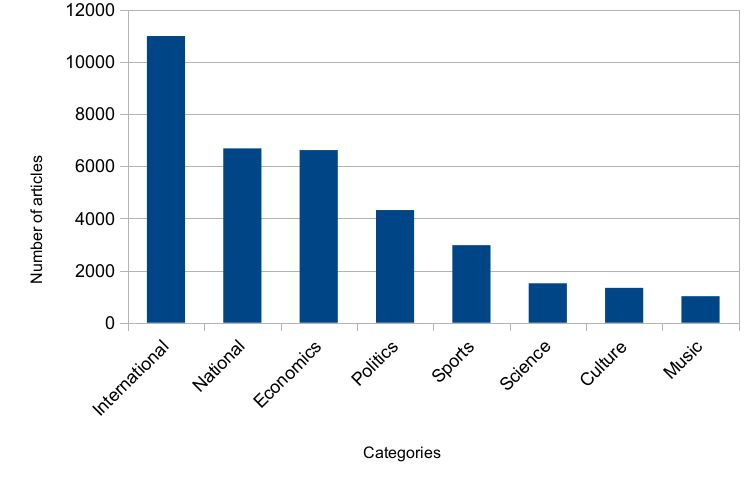
\includegraphics[width=.97\columnwidth]{imgs/articles}}
\caption{Total number of articles retrieved for each category}
\label{fig:articles}
\end{figure}

We them randomly selected, from each category, 700 articles to be used
to train the classifiers, and 200 to be used to evaluate their
performance.

For each article, we had available its contents (title, lead, body)
and several metadata fields (publication date, category, tags, etc). A
truncated JSON representation of an article can be found in
Listing~\ref{lst:article}.


\subsection{Preprocessing the articles}
\label{sec:preproc}

Originally, the dataset was obtained as large MongoDB collection (more
than 2.5 million entries), containing articles from several Portuguese
and international newspapers. The process needed to transform this
collection into data our classifiers could process required querying
the database, exporting the news articles and splitting them into a
train and an evaluation datasets.

The database query selected articles from \texttt{Observador} where
the body had a length greater than 100 characters (to
discard some malformed articles which had an empty body or a body
composed of only a few words), and the categories included at least
one of the most common categories.

For each article returned by the query, the pretitle, title, subtitle
and lead fields, if present, were simply copied to a plain text file,
separated by blank lines. The body field, however, was stored in the
database in HTML format. As such, the HTML tags had to be stripped,
and then it was also added to the plain text file.

The files were then stored in folders, separated by the category.
Furthermore, for each category, 700 articles were allocated to the
train set, and 200 to the evaluation set. These preprocessing tasks
were accomplished using Bash and Node.js scripts.

Both datasets were then loaded into R using the
\texttt{tm}\footnote{\url{https://cran.r-project.org/web/packages/tm/}}
package. Each was then passed to a function responsible for
preprocessing the text of the articles:

\begin{itemize}
    \item the text was converted to lowercase characters
    \item the Portuguese stopwords were removed
    \item diacritics were converted to their normalized form (e.g.
        \framebox{à} $\rightarrow$ \framebox{a})
    \item punctuation signs were removed
    \item numbers were removed
    \item word were stemmed (e.g. \framebox{conseguiram} $\rightarrow$
        \framebox{consegu})
    \item whitespace was removed and the text was tokenized
\end{itemize}

A document-term matrix was then calculated using the
\texttt{DocumentTermMatrix} method from the \texttt{tm} package.
For each of the 5600 documents preset in the train set the matrix
included all the terms which met the following requirements:

\begin{itemize}
    \item the term length was between 3 and 30 characters (to discard
        things like URLs or badly tokenized sentences)
    \item the term appeared in the document at least twice
    \item the term appeared at least in 10 documents
\end{itemize}
The algorithm used to weigh the terms in the matrix was the
\textit{tf-idf}\cite{christopher2008introduction}. The obtained matrix
presented a sparsity of 99\% and contained 3234 distinct terms.

The final step was to remove the sparse terms from the matrix.
This allows to discard terms which might be too specific of the train
set and which might negatively influence the performance of the
classifiers by overfitting them to the train set. Additionally, a
smaller list of terms reduces the execution time of both training and
applying the classifier, and the memory footprint of the classifier.
However, while discarding sparse terms we might end up removing
relevant terms and increase our classifiers error rate.

We used the \texttt{removeSparseTerms} function from the \texttt{tm}
package, and produced three distinct lists of terms:
\begin{description}
    \item[$LT_{90}$] contained terms with 90\% or less sparsity
    \item[$LT_{95}$] contained terms whose sparsity was under 95\%
    \item[$LT_{99}$] contained the terms with a sparsity level below 99\%
\end{description}

\subsection{Classification}

To create the classifiers, we used 5 well knows algorithms: decision
tree (DT), k-nearest neighbors (KNN), naive Bayes (NB), neural network
(NN) and support vector
machine -- with radial kernel (SVM\textsubscript{RK}) and linear
kernel (SVM\textsubscript{LK}).

For the process of training a

We trained each of the classifiers three different times, one for each
list of terms ($LT_{99}$, $LT_{95}$ and $LT_{90}$). Then we evaluated
each trained classifier using the test dataset.

The test dataset contained 1600 documents (200 belonging to each
category) and was preprocessed in a way similar to the train set
(described in the previous section,~\ref{sec:preproc}).  In each
iteration, however, the final list of terms in each test document was
restricted to terms present in the corresponding list of terms
($LT_{99}$, $LT_{95}$ and $LT_{90}$).

\section{Results}
A number of measurements and metrics were calculated regarding the
lists of terms, the classifiers training process and their results in
the evaluation process.

Table~\ref{tab:size} presents the size of each list of terms after
removing the terms whose sparsity was above the corresponding
threshold.

\begin{table}[htbp]
    \vspace{-.5cm}
    \caption{Lists size}
\begin{center}
\begin{tabular}{l|SS}
    & \parbox{6em}{\centering Sparsity\\threshold (\%)}  &
    \parbox{5em}{\centering Number\\of terms}   \\\hline
    $LT_{90}$ &  90                 &  45 \\
    $LT_{95}$ &  95                 & 139 \\
    $LT_{99}$ &  99                 & 912 \\
\end{tabular}
\label{tab:size}
\end{center}
\end{table}

Table~\ref{tab:exectime} presents the execution time for training the
algorithm with the lowest error rate for each list of terms.

\begin{table}[htbp]
    \vspace{-.2cm}
    \caption{Execution times for training}
\begin{center}
\begin{tabular}{l|cr}
    & Algorithm  & \parbox{3em}{\centering Training\\time} \\\hline
    $LT_{90}$    & DT         & 12s  \\
    $LT_{95}$    & KNN        &  3m  \\
    $LT_{99}$    & KNN        & 57m  \\
\end{tabular}
\label{tab:exectime}
\end{center}
\end{table}


Table~\ref{tab:error} presents the error rates obtained for each list
of terms using each of the classifiers, with the value of the best
classifier for each list highlighted in bold.

\begin{table}[htbp]
    \vspace{-.2cm}
    \caption{Error rates}
\begin{center}
\begin{tabular}{l|rrrrrr}
                 & DT            & KNN           & NB   & NN   & SVM\textsubscript{RK} & SVM\textsubscript{LK} \\ \hline
    $LT_{90}$    & \textbf{0.60} & 0.71          & 0.85 & 0.61 & 0.88                  & 0.88                  \\
    $LT_{95}$    & 0.70          & \textbf{0.56} & 0.83 & 0.58 & 0.87                  & 0.87                  \\
    $LT_{99}$    & 0.70          & \textbf{0.35} & 0.87 & 0.76 & 0.87                  & 0.87                  \\
\end{tabular}
\label{tab:error}
\end{center}
\end{table}

Table~\ref{tab:confmat} presents the confusion matrix generated using
the k-nearest neighbors classifier with the $LT_{99}$ list of therms,
with the number of correct classifications for each category
highlighted in bold.

\begin{table}[htbp]
    \caption{Categories confusion matrix ($LT_{99}$ with KNN)}
\begin{center}
\begin{tabular}{l|rrrrrrrr}
& \rotatebox{75}{science}    & \rotatebox{75}{culture}  &
    \rotatebox{75}{sports} & \rotatebox{75}{economics} &
    \rotatebox{75}{international}    & \rotatebox{75}{music}   &
    \rotatebox{75}{national}     & \rotatebox{75}{politics} \\\hline
science       & {\bf 127} & 19        & 1          & 6         & 12       & 24        & 11       & 0 \\
culture       & 5         & {\bf 102} & 2          & 2         & 3        & 79        & 6        & 1 \\
sports        & 1         & 3         & {\bf  168} & 7         & 3        & 14        & 4        & 0 \\
economics     & 5         & 3         & 0          & {\bf 146} & 5        & 17        & 14       & 10 \\
international & 12        & 12        & 7          & 17        & {\bf 90} & 35        & 16       & 11 \\
music         & 0         & 2         & 0          & 0         & 2        & {\bf 184} & 1        & 0 \\
national      & 9         & 9         & 9          & 19        & 15       & 31        & {\bf 88} & 21 \\
politics      & 1         & 3         & 0          & 30        & 8        & 17        & 14       & {\bf 127} \\
\end{tabular}
\label{tab:confmat}
\end{center}
\end{table}

\section{Discussion}

The analysis of the results obtained should take into account other
metrics besides the error rates obtained for each classifier.

The size of the list of terms, for example, gives us an idea of the
memory footprint of a classifier, a parameter which is of the utmost
importance if the goal is to implement a classifier as lightweight as
possible. The training time is also relevant, as shorter training
times give the possibility of retraining the classifiers more often,
allowing them to be updated as the corpus of news articles grows.

Looking at the actual results obtained and represented in
Tables~\ref{tab:size} and \ref{tab:exectime} we can see that $LT_{90}$
has simultaneously the smallest list of terms (45) and the shortest
training time (12 seconds using the decision tree algorithm). However,
$LT_{90}$ also presents the worst error rates, even when looking at
the algorithm which achieved its best results (0.60 using a decision
tree classifier).

On the opposite side, $LT_{99}$ presented the lowest error rates (0.35
using a k-nearest neighbors classifier), but it took almost one hour
to train and used a list comprising 912 terms.

The results obtained confirm that there is a tradeoff between the size
of the list of terms and the training time, on the one hand, and the
classifier error rate, on the other. However, a list of 912 terms
seems to be an acceptable memory footprint for a client side
classifier; additionally, the additional training time would not present
much problems in this scenario, as the classifier would be trained
before hand and thus would not be visible on the client side.

Given the reasonable values for the training time and the size of the
list of terms, and looking to the error rate obtained in each of tests
performed, we can conclude that the best option was to use the largest
list of terms ($LT_{99}$) and the k-nearest neighbors classifier.

It is worth noting that the categories of an article are not mutually
exclusive. In fact, an article can be classified as belonging to more
than one category. This might explain the greater error rates obtained
in the categories \textit{national} and  \textit{international}: one
might argue that these categories correspond less to the topic covered
by the article and are more related to the location of the news
content.

\section{Contributions and Future work}
For copyright reasons, the corpus used to train and evaluate the
classifiers described in this article cannot be shared. All the code
used to process the documents, to implement the classifiers and
evaluate them can be found at\\
\url{http://github.com/andrefs/mapi-msr-categorization}.

The tasks and results previously described already provide useful
insights into this matter. However, the lowest error rate obtained
(0.35), despite already acceptable, might still be improved, either by
trying new algorithms, fine tuning the ones already tested, or by
increasing the train corpus.

We have established that it is in fact possible
to develop a news article classifier which is lightweight enough to be
used (in real time) on the client side of a web application. The
following step will be the actual implementation, probably in the form
of a JavaScript library, of such a classifier.


\section*{Acknowledgment}

André Santos has a PhD scholarship from Fundação para a Ciência e
Tecnologia.

\bibliography{article}
\bibliographystyle{splncs03}

\end{document}
